\chapter{Project Methodology}

% ROUGHLY Outline the conceptual/theoretical framework of the project, the project design and methods. Demonstrate that methodologies are robust and adequately developed.
\section{Development of the BedSAT Inversion Framework}
BedSAT's goal is to leverage a physically informed transfer function with improved understanding of how ice rheology and basal sliding conditions affect the surface expression of subglacial topography. Its development requires the following stages.

\begin{enumerate}
\item{\textbf{Training}}:
BedSAT will be trained and validated using a physically informed (ODSA) synthetic bedrock database (Bedrock Factory) and a data-rich region, such as the Aurora Subglacial Basin, where extensive ice-penetrating radar data of the bed is available for direct comparison.\\
\textbf{Forward Ice Flow Model}:
The forward model of ice dynamics will be configured for the chosen study site, including key model assumptions, such as the choice of ice flow equations and the parameters governing ice rheology. The robustness of the numerical configuration will be confirmed through grid independence testing to ensure that the results are not an artefact of the model's spatial resolution.\\
\textbf{Inversion Pre-processing}:
The primary observational inputs for the model will be satellite-derived surface velocity, surface elevation~\cite{Rignot_2011, REMA} and ice thickness~\cite{Young_2011, ICECAP}. A critical pre-processing step will involve filtering high-frequency noise (e.g., aeolian features) from the surface data to ensure that the glaciological signal from the underlying bed is isolated.

\item{\textbf{Inverse Modelling to Estimate Bed Topography}}:
The core of the BedSAT is the inversion. BedSAT will iteratively adjust an initial estimate of the bed topography, aiming to minimize the mismatch between the forward model's simulated surface velocities and the satellite-observed velocities.

\item{\textbf{Validation and Sensitivity Analysis}}:
BedSAT's performance will be rigorously evaluated. First, the inverted bed topography will be directly validated against the "ground-truth" radar-derived bed maps for the study region. Second, a series of sensitivity analyses will be conducted to quantify the model's robustness. These tests will systematically alter key assumptions, such as the rheological parameters for different regions, to determine their impact on the final inverted topography and to establish the uncertainty bounds of the framework's results.
\end{enumerate}

\section{ODSA's Landscape Classification Vector}\label{vector}

To inform the synthetic bedrock database that will be used in the training, we need bed morphometric statistics to describe a landscape class. We apply ODSA to seven reference regions as proof of concept (see Fig.~\ref{fig:7regions}), quantifying how well the flight lines sample their survey footprint.

\begin{figure}
    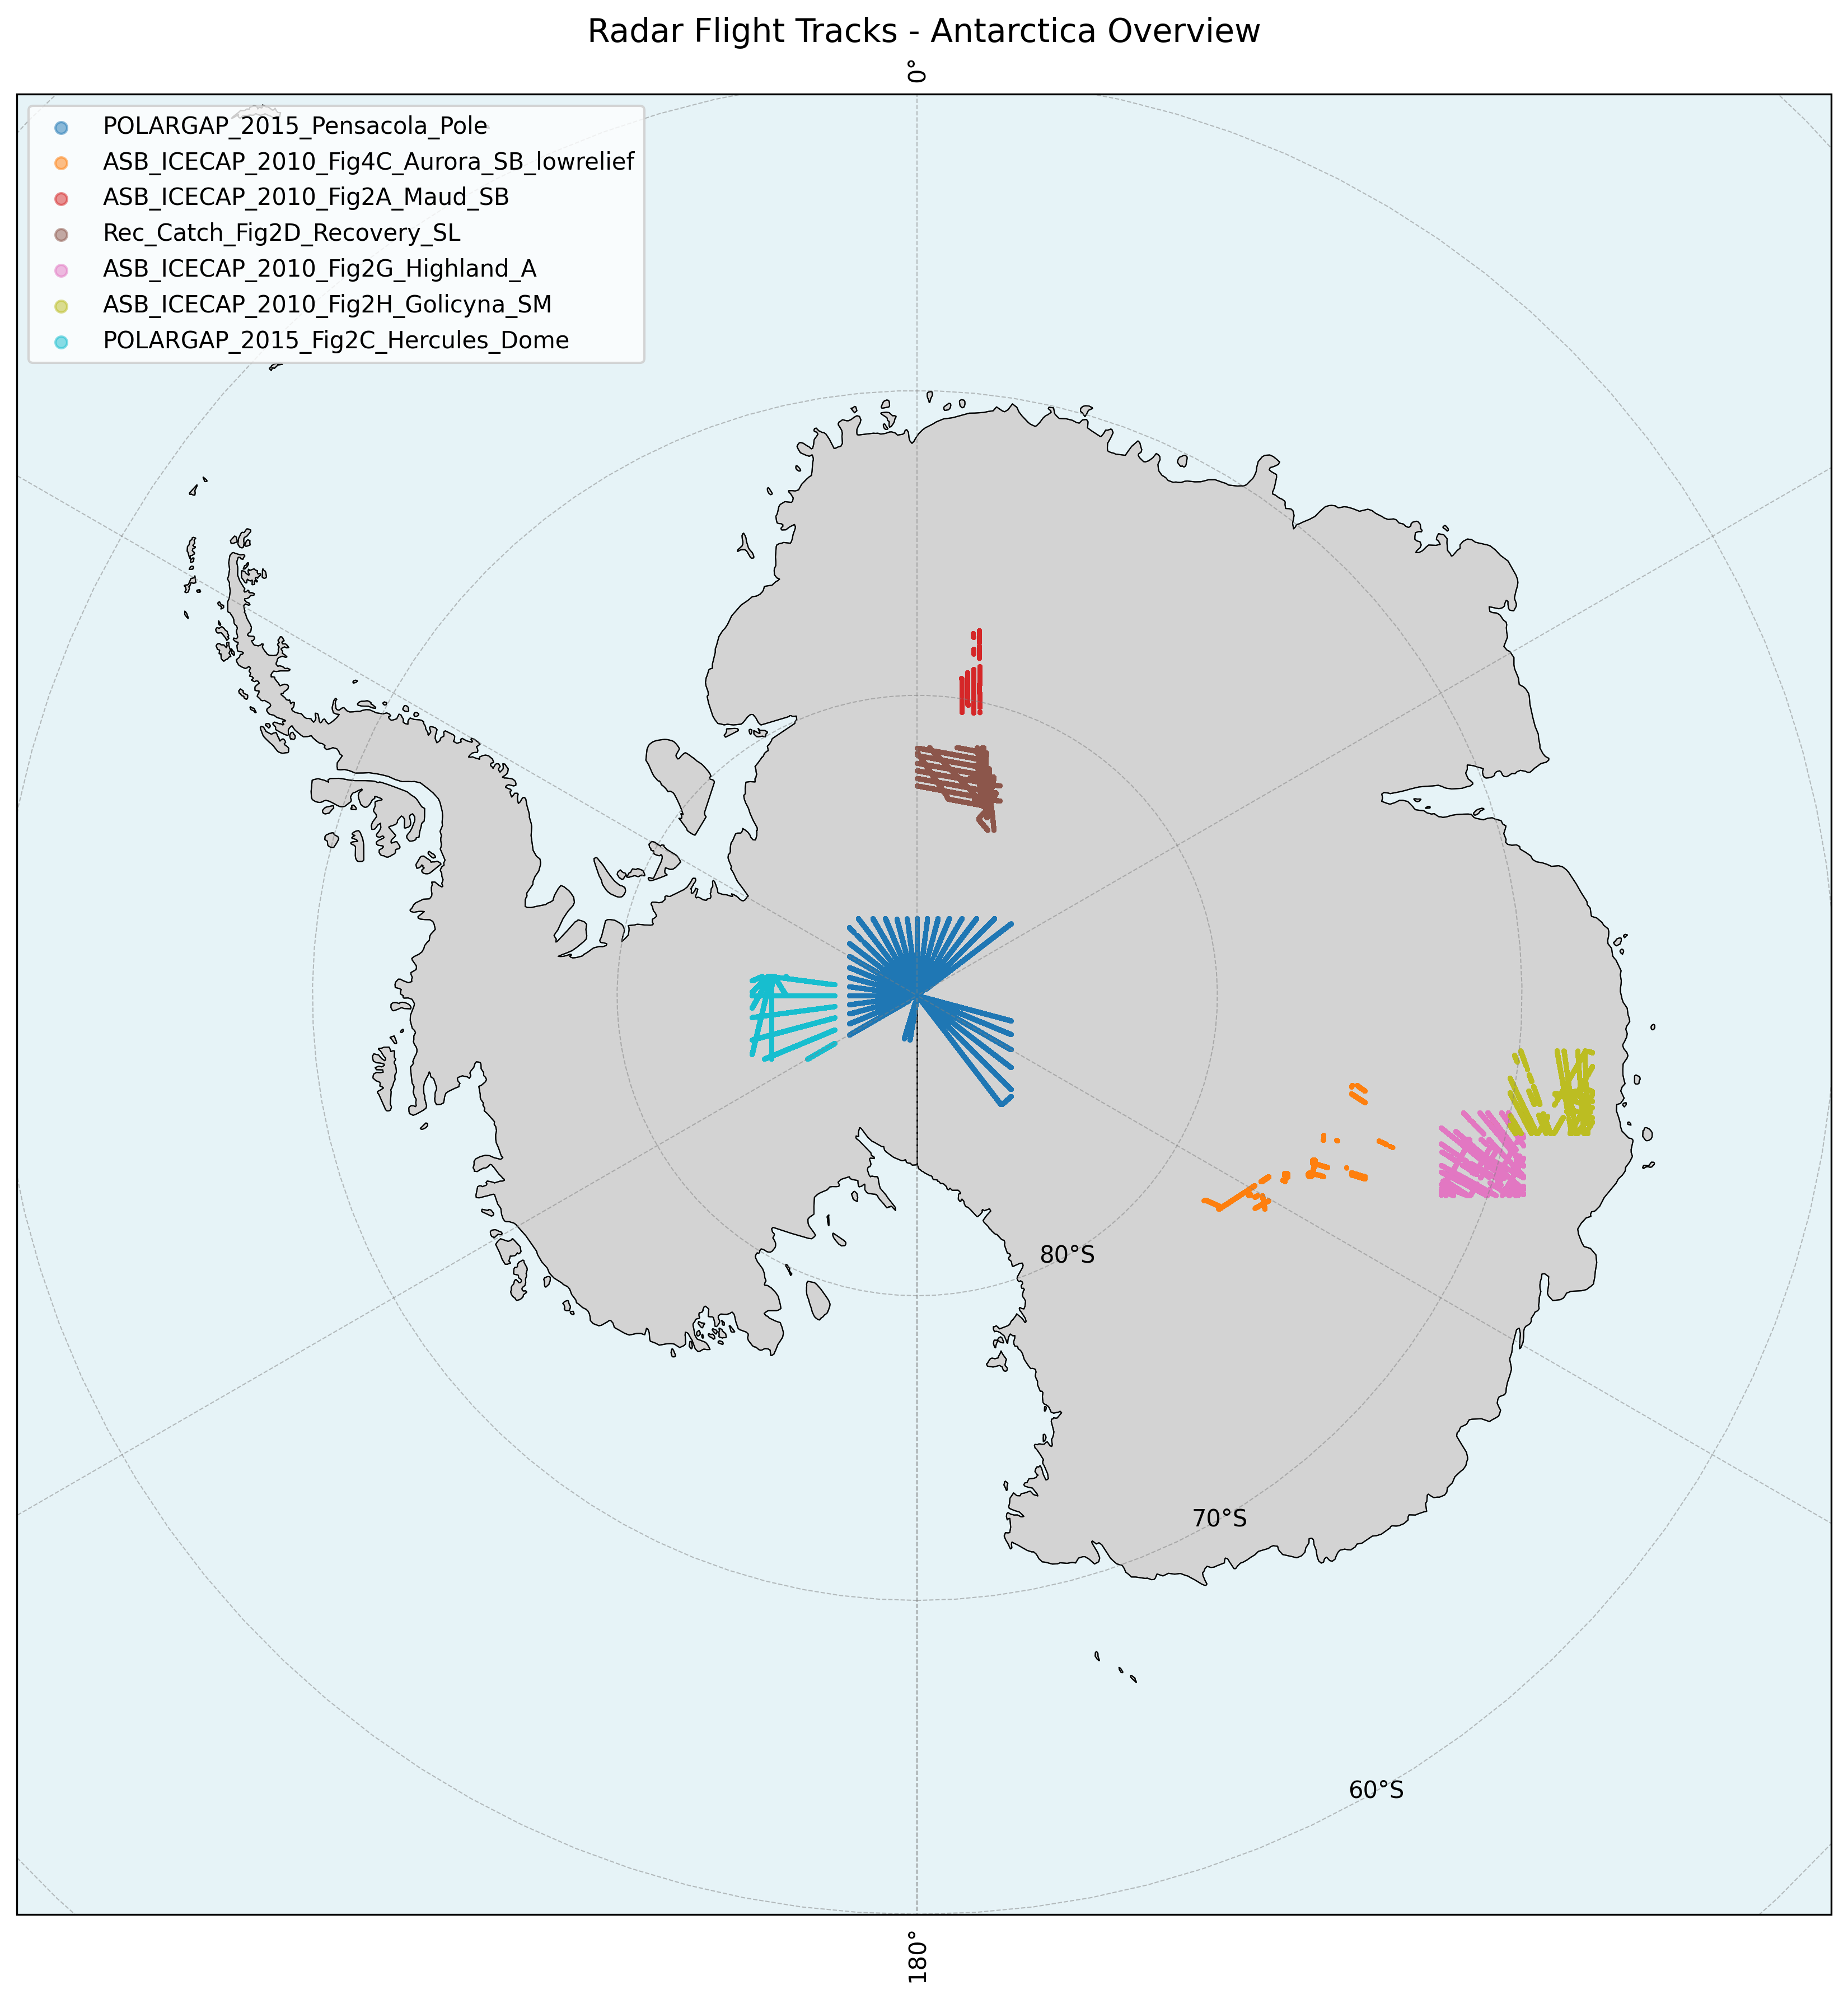
\includegraphics[scale=0.58]{figures/antarctica_tracks_overview.png}
    \caption{The seven RES survey regions we analysed with ODSA. Five regions use the PS71 boxes from~\cite{Ockenden_2025_data}. The Aurora low-relief region is restricted to the low-relief cells of the Ockenden classification, and the Pensacola Pole Basin region uses a box that we defined.} 
    \label{fig:7regions}
\end{figure}

Our proposal is that to bound subglacial landscape class it is necessary to have multiple measured statistics that characterise different landscape properties. ODSA's landscape vector carries 11 elements measured per window. Four classify and seven do not. Each classifier carries an uncertainty envelope of two standard deviations at either side of the measured value, taken from the spectral fit covariance in the case of the roughness slope ($\beta$) and from measurement error budgets for relief, velocity and elevation. The landscape vector provides the morphometric statistics that the Bedrock Factory suite will take as inputs to generate synthetic beds at ice-sheet model resolution.

\begin{table}[H]
\centering
\caption{Classification axes of the landscape classification vector}
\label{tab:axes}
\begin{tabularx}{\textwidth}{l p{4.0cm} X}
\toprule
\textbf{Category} & \textbf{Variable} & \textbf{Description/Thresholds} \\
\midrule
\textbf{Classifiers} 
  & \texttt{$\beta$} & Slope of the bed power spectrum over the fitted band. A measure of bed roughness: low $\beta$ distributes power to the short wavelengths; high $\beta$ concentrates it at long wavelengths.  Literature reported values range from around 1.5 on exposed crystalline terrain to above 2.5 on sedimentary beds~\cite{Bingham_2009} with thawed beds in northern Greenland averaging 2.48 against 2.08 when frozen~\cite{Jordan_2017}. \\
  \addlinespace[0.5em]
  & \texttt{relief\_m} & Elevation range within a window, calculated as $\max\mathrm{(bed)} - \min\mathrm{(bed)}$ over the raw 50 km profile, in metres. It gives the amplitude of the largest structure a window contains. Regional slope enters the range directly. Relief class thresholds are set to flat: $<350~\mathrm{m}$; mountainous: $\geq~800~\mathrm{m}$~\cite{Ockenden_2026}; while values in between these are labelled as subdued. \\
  \addlinespace[0.5em]
  & \texttt{measures\_speed\_mean} & Mean MEaSUREs InSAR surface speed at the window's track points, in m/yr, sampled over the same points that enter the spectral fit. Bands are \texttt{very\_low} ($<5$), \texttt{low} ($5$ to $\leq10$), \texttt{moderate} ($10$ to $\leq50$) and \texttt{fast} ($>50$), anchored on the bimodality in~\cite{Rignot_2011}. Each window carries a sampled error from the \texttt{ERRX/ERRY} fields of that product.\\
  \addlinespace[0.5em]
  & \texttt{bed\_elev\_mean} & The mean bed elevation within a window, in metres above present-day sea level. Class thresholds are set to submerged: $\leq~0~\mathrm{m}$; elevated at $\geq~1000~\mathrm{m}$, and emerged for values in between. Supported by~\cite{Rippin_2014, Frederick_2016}. \\
\bottomrule
\end{tabularx}
\end{table}

\begin{table}
\centering
\caption{Continuous descriptors of the landscape classification vector}
\label{tab:descriptors}
\begin{tabularx}{\textwidth}{l p{4.0cm} X}
\toprule
\textbf{Category} & \textbf{Variable} & \textbf{Description/Thresholds} \\
\midrule
\textbf{Descriptors} 
  & \texttt{A\_1km} & Intercept of the bed power spectrum at a $1~\mathrm{km}$ reference wavelength. It gives shape and magnitude of the roughness and fixes the level inside the fitted wavelength band. It carries a propagated uncertainty that includes the slope and intercept covariance. \\
  \addlinespace[0.5em]
  & \texttt{rms\_roughness} & Root mean square of the window's detrended elevation residuals, in metres. It gives the amplitude of the topography with the regional ramp removed, which distinguishes it from relief. It is retained for comparability with the space-domain roughness literature rather than as a separate degree of freedom. Supported by~\cite{Frederick_2016}. \\
  \addlinespace[0.5em]
  & \texttt{$\eta$\_wavelength\_m} & Characteristic wavelength for the window, in metres, following~\cite{Li_2010}. It is a weighted harmonic average of the square of the wavelength at each frequency in the band with the spectrum as the weight. \\
  \addlinespace[0.5em]
  & \texttt{$\xi$\_band} & Integral of the bed power spectrum over the characteristic wavelength. It is a band-limited variance spanned from $300~\mathrm{m}$ to $1200~\mathrm{m}$, in $\mathrm{m^2}$~\cite{Li_2010}. Supported by~\cite{King_2007, Spagnolo_2017}. \\
  \addlinespace[0.5em]
  & \texttt{hill\_count} & Number of distinct local maxima in the window's detrended bed profile, similar to the bumpiness metric by \cite{Ockenden_2026} but in transect form (1D). A point counts if it is the maximum of a $5~\mathrm{km}$ box centred on it and the box relief exceeds $20~\mathrm{m}$; adjacent flagged points count once and maxima touching a window edge are dropped. Two hills must be at least $2.5~\mathrm{km}$ apart, so the count cannot exceed $10$ per $50~\mathrm{km}$ window. \\
  \addlinespace[0.5em]
  & \texttt{skewness} & Third standardised moment of the window's detrended, untapered bed elevation residuals (bias-corrected). Positive values imply narrow highs on a broad low base, negative values mean narrow lows cut into a broad high surface, following the qualitative hills-against-troughs distinction in~\cite{Sugden_1978}. It is the only phase-asymmetry information in the vector.\\
  \addlinespace[0.5em]
  & \texttt{kurtosis} & Excess kurtosis of the window's detrended, untapered bed elevation residuals (bias-corrected). Positive values mean a few extreme highs or lows against a flat background, negative values mean a flat-topped or evenly spread distribution.\\
\bottomrule
\end{tabularx}
\end{table}

